\section{Dont cross the streams}
Consider the PDE $\partial_x u + 2x\partial_y u  = 0$ on the domain $y>0$ with the boundary condition $u(x,0) = g(x)$
\begin{question}
  \textbf{(a)} Show that the boundary hyperplane $\{y=0\}  $ is non-characteristic at $(x,0)$, except for $x=0$.
\end{question}
\begin{solution}
Consider the PDE as a function $F(\frac{\partial u}{\partial x},\frac{\partial u}{\partial y},u(x,y),x,y)=0$   then we need to show that : 
\begin{align*}
  \partial_{p_{1}} F(p_{0},p_{1},z,x,y) \neq 0
.\end{align*}
In our case : 
\begin{align*} 
  \partial_{p_{1}} F(p_{0},p_{1},z,x,y)  = \partial_{p_{1}} \left( p_{0} + 2x p_{1} \right)   = 2x
.\end{align*}
Which as required is non zero on $(x,0)$ except for $x=0$
\end{solution}
\begin{question}
  \textbf{(b)}  What condition does the PDE impose on the boundary data g at the point $(0,0)$
\end{question}
\begin{solution}
 At the point $(0,0)$ we know $F(d \frac{g(0)}{dx},p_{1},g(0),0,0) = 0$ but 
 \begin{align*}
  F(d \frac{dg(0)}{dx},p_{1},g(0),0,0) = \frac{dg}{dx}(0) + 2*0*p_{1} =  \frac{dg}{dx}(0) = 0
 .\end{align*}
 The PDE requires g to be constant at $(0,0)$
\end{solution}
\begin{question}
  \textbf{(c)} Determine the characteristic curves of this PDE.
\end{question}
\begin{solution}
 Consider $z(s) = u(x(s),y(s))$  then : 
 \begin{align*}
   z'  = \partial_x u x' + \partial_y y' 
 .\end{align*}
 Choosing $x' = 1 $ and $y' =  2x$ aligns with the PDE such that  
 \begin{align*}
   x(s) &= s +x_{0} \\
   y(s) &= 2xs + y_{0}
 .\end{align*}
 Considering the initial condition 
 \begin{align*}
  z(0) = u(x(0),y(0)) =  u(x_{0},0)
 .\end{align*}
 Meaning $y(s) = 2xs$ this leads to : 
 \begin{align*}
   z(s) = u(x_{0}+s,2xs) = g(x_{0})
 .\end{align*}
 For $(x,y)$ we get : 
 \begin{align*}
   x_{0} &= x-s  \\
   s     &= \frac{y}{2x}
 .\end{align*}
 Such that : 
 \begin{align*}
  u(x,y)  = g(x-\frac{y}{2x})
 .\end{align*}
\end{solution}
\begin{question}
 By considering the $y$-derivative of u on the boundary hyperplane, show that there is no $\mathcal{C}^{1} $ solution with the initial data $g(x) = x$
\end{question}
\begin{solution}
% On the boundary hyperplane $H = \{y=0\}  $ we have by (a) that it is non characteristic at $(x,0)$ except for $x=0$ 
% This means that : 
% \begin{align*}
%   \frac{\partial F}{\partial p_{1}}(\frac{dg(0)}{dx},p_{1},z,0,0) = 0 
% .\end{align*}
% Which requires $\frac{dg}{dx}$ to be constant ? idk dude, i think the issue is that g needs to be constant but it isnt
By (b) we know that the PDE requires $g'= 0$ at $(0,0)$ but for initial data $g(x) = x $ we get $\frac{dg}{dx}(0) = 1 \neq 0$, such that no $\mathcal{C}^{1} $ solution may exist,
other way is using that $H = \{y=0\}  $ is non-characteristic at $(0,0)$
\end{solution}
\section{Its just a jump to the left}
We consider the IVP from Example 1.10., as we saw for small t the method of characteristics gives a unique solution
\begin{align*}
  u_{t<1}(x,t) = \begin{cases}
    1 &\text{ for } x<t\\
    \frac{x-1}{t-1} &\text{ for } t\le x < 1\\
    0 &\text{ for } 1\le x\\
  \end{cases}
.\end{align*}
\begin{question}
  \textbf{(a)}  Derive this solution for yourself for extra practice
\end{question}
\begin{solution}
  We consider Burgers equation $\dot{u}(x,t) + u(x,t)\frac{\partial u}{\partial x}(x,t) =0  $  for $(x,t) \in  \mathbb{R} \times  \mathbb{R}^{+} $
  with the following continuous initial values $u(x,0) = g(x)$ and 
  \begin{align*}
    g(x) = \begin{cases}
      1 &\text{ for } x\le 0 \\
      1-x &\text{ for } 0 \le x < 1 \\
      0 &\text{ for } 1 \le x
    \end{cases}
  .\end{align*}
  Deriving the characteristic equations by setting $z(s) = u(x(s),s)$ 
  \begin{align*}
    z' = \partial_x u x' + \partial_t u 
  .\end{align*}
  such that by choosing $x' = u $ 
  \begin{align*}
    z' = 0
  .\end{align*}
  i.e z is constant such that 
  \begin{align*}
    x(s) = x_{0} + z_{0}*s
  .\end{align*}
With $z_0 =u(x_{0},0) = g(x_{0})$ such that for arbitrary $(x,t) \in  \mathbb{R} \times  \mathbb{R}^{>0} $  we want to evaluate which characteristic they lie on 
i.e the value of $x_{0}$, we do this by first considering the shape of our characteristics : 
\begin{align*}
  x+g(x)*t = \begin{cases}
    x+1*t &\text{ for } x\le 0 \\
    x-t(1-x) &\text{ for } 0 \le  x < 1\\
    x &\text{ for } 1\le x
  \end{cases}
.\end{align*}
We know that to get a unique solution the characteristics cannot cross, for $t=1$ we get a crossing such that 
we need to restrict our solution to $t<1$, to get our desired $x_{0}$ we take the inverse of the above mapping (invertible cause stricly monotone for $t<1$ ) with 
\begin{align*}
  y \mapsto \begin{cases}
    y-t &\text{ for } y\le t \\
    \frac{y-t}{1-t} &\text{ for } t <  x < 1\\
    y &\text{ for } 1\le x
  \end{cases}
.\end{align*}
Therefore we get the desired solution :
\begin{align*}
  u_{t<1}(x,t) =  \begin{cases}
    x-t &\text{ for } y\le t \\
    \frac{x-1}{t-1} &\text{ for } t <  x < 1\\
    0 &\text{ for } 1\le x
  \end{cases}
.\end{align*}
\end{solution}
\begin{question}
  \textbf{(b)} Draw the corresponding characteristics diagram in the $(x,t)$- plane  
\end{question}
\begin{solution}
    \begin{figure}[H]
     \centering 
     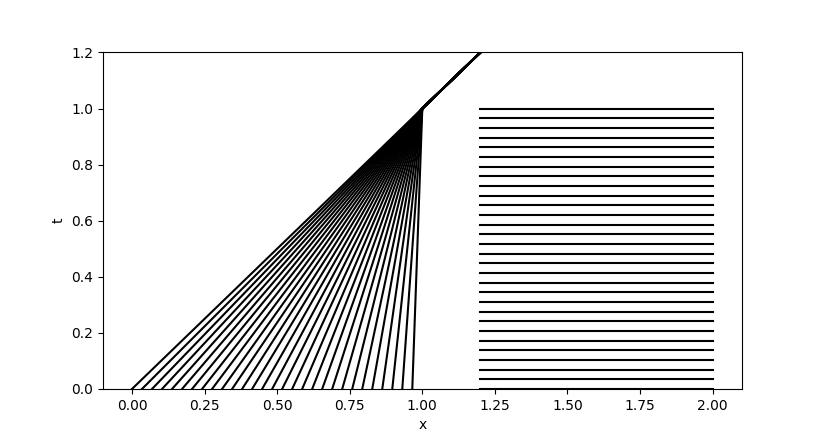
\includegraphics[scale=0.5]{figures/sheet_4_char.png} 
   \end{figure}
\end{solution}
\begin{question}
  \textbf{(c)} Describe the graph of disontinuities y(t). Compute the Rankine-Hugonoit condition for v. 
\end{question}
\begin{solution}
 The disontinuity occurs when our solution jumps from 0 to 1, this occurs when $x \uparrow t$  or $x \downarrow t$, i.e along the line $y(t) = t$, we compute the condition by : 
 \begin{align*}
  \dot{y} = \frac{f(u^{r} )-f(u^{l} )}{u^{r} - u^{l}  } 
 .\end{align*}
 In our case $f = \frac{1}{2}u^{2} $ and $\dot{y} = 1 $ 
 \begin{align*}
  1 \neq  \frac{0 - \frac{1}{2}}{-1} = \frac{1}{2}
 .\end{align*}
 Such that the condition is not fulfilled  
\end{solution}
\begin{question}
  \textbf{(d)} How much mass (i.e the integral of v over x) is being lost in the system described by v for $t>1$
\end{question}
\begin{solution}
 Integrating for fixed t  
 \begin{align*}
   F_{[a,b]}(t) = \int_{a}^{b}  v(x,t) dx &= \int_{a}^{t} v(x,t) dx + \int_t^{b}  v(x,t) dx  \\
                           &= \int_{a}^{t} 1 dx   = t-a
 .\end{align*}
 i.e $F' = 1$  the mass over $[a,b]$ changes by 1 for every increase in t. 
 %By the scalar conservation property we know that on the compact invertval $x \in [t-\epsilon ,t+\epsilon ]$ the change in mass is described by  ? 
 % \begin{align*}
 %  f(u(t-\epsilon ,t)) - f(u(t+\epsilon ,t)) = \frac{1}{2}*1^2 - 0 =  \frac{1}{2}
 % .\end{align*}
\end{solution}
\section{You're not in traffic, you are traffic}
In this question we look at an equation similar to Burgers’ equation that describes traffic. Let
$u$ measure the number of cars in a given distance of road, the car density. We have seen that
$f$ should be interpreted as the flux function, the number of things passing a particular point.
When there are no other cars around, cars travel at the speed limit $s_m$. When they are bumper-
to-bumper they can’t move, call this density $u_m$.
\begin{question}
  \textbf{(a)} What properties do you think that f should have? Does $f(u)= s_m u (1-\frac{u}{u_m})$ have these properties 
\end{question}
\begin{solution}
 The flux f should describe the flow of cars given the density of cars on any given stretch, 
 to properly describe this f needs to consider the case of 0 cars i.e density $u=0$  and the case $u=u_m$.
 The flux of traffic f should be a function of the number of cars u and the speed each car moves at i.e : 
 \begin{align*}
  f(u)= u*s(u)
 .\end{align*}
 Where we know that $s'(u)\rvert_{u=0} = s_m$ and $s'(u) \rvert_{u=u_m} = 0$ i.e 
 \begin{align*}
  s(u)  = s_m * (1- \frac{u}{u_m})
 .\end{align*}
plugging into $f$ gives the described function
\end{solution}
\begin{question}
  \textbf{(b)}  Find a function f that meets your condition or use the f from the previous part, and write down a PDE to describe the traffic flow
\end{question}
\begin{solution}
  We take $f(u)=u*s(u)$ as previously defined and model using a conservation law 
  \begin{align*}
    \dot{u}   = -\frac{\partial f(u)}{\partial x} 
  .\end{align*}
  i.e the change of density on any given stretch  in t should be proportional to the fluxes change in x 
\end{solution}
\begin{question}
  \textbf{(c)}  Find all solutions that are constant in time 
\end{question}
\begin{solution}
  Solutions constant in time implies 
  \begin{align*}
    \dot{u}  = 0
  .\end{align*}
  such that 
  \begin{align*}
    0 = -\partial_x f(u) \implies 0 = - \partial_u f*\partial_x u
  .\end{align*}
  Where 
  \begin{align*}
    \partial_u f =  -u*\frac{s_m}{u_m} + s_m(1-\frac{u}{u_m}) = s_m*(1-2\frac{u}{u_m} )
  .\end{align*}
  Which gives 
  \begin{align*}
    0 = \partial_xu*s_m*(1-2\frac{u}{u_m})
  .\end{align*}
  Such that any constant solution must have 
  \begin{align*}
    \partial_xu = 0
  .\end{align*}
  or 
  \begin{align*}
    1-2 \frac{u}{u_m}  = 0  \implies   1 = 2 \frac{u}{u_m} \implies \frac{u_m}{2} = u
  .\end{align*}
  Meaning all constant functions $u$ solve the PDE.
\end{solution}
\begin{question}
  \textbf{(d)}  Consider the situation of a traffic light at $x=0$: to the left of the traffic light , the cars 
  are queued up at maximum density. To the right of the trafic light, the road is empty. Now, at time $t=0$ the traffic light turns green.
  Give a discontinuous solution that obeys the Rankine-Hugonoit condition as well as a continuous solution
\end{question}
\begin{solution}
  We have $u(-\epsilon ,t=0) = u_m$  and $u(\epsilon,t=0) = 0 $, 
  The Rankine-Hugonoit condition is given by 
  \begin{align*}
  \dot{y} = \frac{f(u^{r}(y,t) )-f(u^{l}(y,t) )}{u^{r}(y,t) - u^{l}(y,t)  } 
  .\end{align*}
  Where $\lim_{x \uparrow y(t)} u(x,t) =  u^{l}(y,t) $ , $u^{r} $ analog, the jump occurs  at $t=0$ when the light 
  switches to green and cars go from full stop to full speed, i.e $u^{r}(y,t)=0 $ and  $u^{l}(y,t)=u_m $
  \begin{align*}
    \dot{y} = \frac{f(u^{r} ) - f(u^{l} )}{u^{r} - u^{l}  }  = \frac{f(0)-f(u_m)}{0-u_m} = \frac{0 - 0}{-u_m} = 0
  .\end{align*}
  discontinuous solution 
  \begin{align*}
    u(x,t) = \begin{cases}
      0 &\text{ if } x\ge t \\
      u_m &\text{ if } x<t\\
    \end{cases}
  .\end{align*}
  By (c) on both sides of $y(t) = 0$ u is a solution and fulfills the Rankine-Hugonoit condition (hätte eigentlich gesagt es sollte $x>t$ und $x<t$ aber was is bei $x=t$)\\[1ex]
  For a continuous solution consider the characteristic curves by 
  \begin{align*}
    x(t) = x_{0} + t f'(g(x_{0})) \implies x(t) = x_{0} + t*(s_m(1-2 \frac{g(x_{0})}{u_m}))
  .\end{align*}
  Consider for $s_m = 1 , u_m = 2$ (doenst matter really)
  \begin{align*}
   x(t) = x_{0} + t*(1-g(x_{0})) 
  .\end{align*}
  Initial condition $u(x_{0},0) = g(x_{0})$ where we know that $g(-\epsilon ) = 2$ and $g(\epsilon ) = 1$ furthermore we know 
  % that any solution $u(x,t)$ is constant along the lines $x(t) = x_{0} + t*(1-g(x_{0})) $ take $x_0 = 0 $ 
  % \begin{align*}
  %   \frac{x}{t} =(1-g(x_{0}))
  % .\end{align*}

\end{solution}

